% Per-Sample Hessian Trace as Annotation-Free Minority Group Proxy
% Overleaf-compatible LaTeX project (article class fallback — ICML 2025 style)
% To use ICML style: add icml2025.sty and replace \documentclass{article} with \usepackage{icml2025}
\documentclass[10pt,twocolumn]{article}

\usepackage[margin=1in]{geometry}
\usepackage{microtype}
\usepackage{graphicx}
\usepackage{booktabs}
\usepackage{hyperref}
\usepackage{amsmath}
\usepackage{amssymb}
\usepackage{multirow}
\usepackage{listings}
\usepackage{xcolor}
\usepackage{natbib}

\lstset{
  basicstyle=\small\ttfamily,
  breaklines=true,
  frame=single,
  backgroundcolor=\color{gray!10}
}

\title{\textbf{Per-Sample Hessian Trace as an Annotation-Free\\Minority Group Proxy Under ERM Training}}
\author{Anonymous}
\date{}

\begin{document}

\maketitle

\begin{abstract}
Empirical risk minimization (ERM) on spuriously correlated data creates systematic accuracy gaps between majority and minority groups, but identifying minority-correlated training samples without group annotations remains an open problem. We propose measuring per-sample last-fc Hessian trace --- estimated via $K{=}50$ Hutchinson probes using \texttt{torch.func} \texttt{vmap+vjp} --- as an annotation-free proxy for minority group membership in ERM-trained neural networks. On Waterbirds, 4/5 random seeds achieve AUROC$\geq$0.85 for minority membership prediction at the epoch $t^*$ of maximum trace ratio, with epoch-0 AUROC$<$0.70 confirming the signal is ERM-induced rather than inherited from ImageNet pretraining. However, investigation of the mechanism reveals that minority training confidence saturates to $\geq$0.967 at $t^*$ (range: 0.9678--0.9999 across seeds) --- effectively equal to majority --- refuting the predicted confidence-differential mechanism. The trace asymmetry must therefore arise from the feature-norm channel ($\|x_i\|^2$), consistent with \cite{labonte2024spectral}'s spectral imbalance result at the group level. We present the first per-sample second-order annotation-free minority proxy achieving AUROC$>$0.85, alongside a principled falsification of its expected mechanism.
\end{abstract}

\section{Introduction}

We trained ResNet-50 on Waterbirds and found that --- without any group labels --- the curvature of the loss surface around each training sample reveals minority group membership with AUROC 0.85--0.90 in 4/5 random seeds (mean AUROC 0.89 across the 4 passing seeds). But when we investigated \emph{why}, the expected mechanism was absent: by the time the curvature signal peaks, minority samples are classified just as confidently as majority samples. The method works --- but not for the reason we expected.

This puzzle sits at the intersection of two long-standing problems in robust machine learning. The first is spurious correlations: models trained with empirical risk minimization (ERM) on real-world datasets learn to exploit incidental statistical associations between input features and labels. On Waterbirds \cite{sagawa2019distributionally}, a ResNet-50 trained with ERM achieves 97\% average accuracy but only 72\% worst-group accuracy --- minority groups (e.g., landbirds on water backgrounds) suffer because the model relies on background rather than bird shape. The second problem is annotation burden: the most effective mitigation methods, such as deep feature reweighting (DFR) \cite{kirichenko2022last}, require a balanced held-out validation set with explicit group labels --- a resource unavailable in many practical settings.

Annotation-free alternatives --- Just Train Twice (JTT) \cite{liu2021just}, SELF \cite{labonte2023towards}, EVaLS --- proxy minority membership through first-order signals: which samples are misclassified, or which have the highest loss. These methods improve over ERM without group labels, but they operate on signals that are fundamentally insensitive to \emph{how} the model encodes spurious features in its loss landscape geometry.

We ask: does the second-order geometry of the loss surface carry distinct information about minority group membership? Specifically, we measure the per-sample Hessian trace of the last fully-connected layer --- computed via $K{=}50$ Hutchinson estimation using \texttt{torch.func} \texttt{vmap+vjp} --- at six training checkpoints ($t\in\{0,1,5,10,20,50\}$) over five random seeds, and ask whether this trajectory discriminates minority from majority samples.

The measurement protocol is motivated by two theoretical results. \cite{labonte2024spectral} show that minority group covariance matrices have larger spectral norm than majority groups --- a group-level prediction of systematic feature-norm inequality ($\|x_i\|^2$) that would elevate per-sample Hessian traces for minority samples. \cite{labonte2026phase} prove that SGD on spurious data learns the spurious feature first (Phase I) before the core feature (Phase II), predicting a transient differential in loss landscape curvature between majority (which gain confidence rapidly via the spurious shortcut) and minority (which do not).

Our existence experiment (H-E3) confirms the signal: 4/5 seeds achieve AUROC$\geq$0.85 for minority membership prediction at $t^*$ (the epoch maximizing the trace ratio $R(t) = \overline{\text{trace}}_{\text{min}} / \overline{\text{trace}}_{\text{maj}}$), with epoch-0 AUROC$<$0.70 in all seeds --- confirming that ERM training creates the signal, not the pretrained ImageNet initialization. The Hutchinson estimator is stable (coefficient of variation CV$<$3\% for all seeds), establishing $K{=}50$ as sufficient for the last-fc layer of ResNet-50.

Our mechanism experiment (H-M1) produces the puzzle. The original mechanistic explanation --- that minority samples remain near the decision boundary ($p_i\in[0.3,0.7]$) throughout Phase I, keeping the confidence-entropy term $p_i(1-p_i)$ in $\text{Tr}(H_i^{fc}) \propto \|x_i\|^2 p_i(1-p_i)$ large --- is directly falsified. At $t^*$, minority training-set confidence is 0.9678--0.9999 across all seeds: fully saturated, not boundary-straddling. The confidence channel is inactive. A transient differential does exist at epoch 1 (seed 1: $p_{\min}=0.827$ vs $p_{\text{maj}}=0.972$), consistent with Phase I theory, but it disappears before $t^*$.

The trace signal at $t^*$ must therefore arise from the $\|x_i\|^2$ feature-norm channel --- systematic differences in the penultimate-layer representation norms between minority and majority samples, consistent with \cite{labonte2024spectral}'s spectral imbalance finding. This is an unverified but testable candidate mechanism that we identify as the primary direction for future mechanistic investigation.

Our contributions are:

\begin{enumerate}
\item \textbf{Empirical existence result:} First experimental evidence that per-sample last-fc Hessian trace ($K{=}50$ Hutchinson via \texttt{vmap+vjp}) achieves AUROC$\geq$0.85 for minority membership detection in ERM-trained ResNet-50 on Waterbirds across 5 random seeds, with epoch-0 control confirming ERM emergence (Section~\ref{sec:results}).

\item \textbf{Principled falsification of the confidence-differential mechanism:} Direct refutation of the sustained decision-boundary hypothesis ($p_{\text{minority}}\in[0.3,0.7]$ at $t^*$) on training-set data, identifying the feature-norm channel ($\|x_i\|^2$) as the likely driver (Section~\ref{sec:discussion}).

\item \textbf{Practical confirmation:} $K{=}50$ Hutchinson is the minimum stable setting for last-fc ResNet-50 (CV$<$3\%), with the epoch-0 control serving as a reliable pretrained-artifact detector (Section~\ref{sec:experiments}).
\end{enumerate}

The remainder of the paper is organized as follows. Section~\ref{sec:related} reviews related work. Section~\ref{sec:method} describes our methodology. Section~\ref{sec:experiments} details the experimental setup. Section~\ref{sec:results} presents results. Section~\ref{sec:discussion} discusses findings, limitations, and the mechanism puzzle. Section~\ref{sec:conclusion} concludes.

\section{Related Work}
\label{sec:related}

\subsection{Spurious Correlations and Group Robustness}

Spurious correlations --- statistical associations between features and labels that do not reflect causal structure --- cause ERM-trained models to fail systematically on minority groups \cite{sagawa2019distributionally}. The Waterbirds benchmark \cite{sagawa2019distributionally} isolates this: bird labels are spuriously correlated with backgrounds, creating four groups (2 class $\times$ 2 background) with dramatically different ERM performance. Distributionally robust optimization (DRO) directly targets worst-group accuracy but requires group annotations at training time \cite{sagawa2019distributionally}.

\subsection{Annotation-Required Methods: DFR}

The most effective post-hoc approach is deep feature reweighting (DFR) \cite{kirichenko2022last}: retrain only the last layer on a balanced held-out validation set, keeping ERM-pretrained features frozen. DFR achieves WGA$\approx$88--90\% on Waterbirds with a small balanced set. \cite{hill2025unreasonable} explain DFR's effectiveness as implicit group-balancing: when the retraining set overrepresents minority samples, the final classifier learns to rely on causal features rather than spurious shortcuts. However, DFR's key limitation is the requirement for explicit group annotations in the balanced set --- a requirement our work aims to relax.

\subsection{Annotation-Free Proxies: First-Order Signals}

The annotation-free direction emerged with Just Train Twice (JTT) \cite{liu2021just}: identify misclassified samples after a first ERM run, upweight them, and retrain. JTT achieves WGA$\approx$80--84\% on Waterbirds without group labels. SELF \cite{labonte2023towards} refines this by combining misclassification-based proxy selection with self-training, reaching WGA$\approx$82--87\%. EVaLS uses loss-value thresholding as the proxy signal. All of these methods share a fundamental constraint: they operate on first-order signals --- the model's output or loss --- and are insensitive to loss landscape geometry. They capture whether a sample is hard, not \emph{why} it is hard in terms of the curvature of the loss surface around it.

Our work proposes the first second-order annotation-free proxy: per-sample Hessian trace of the last-fc layer. This signal is orthogonal to loss and misclassification and carries information about the differential curvature created by spurious feature exploitation --- information that first-order signals discard.

\subsection{Loss Landscape Geometry and Hessian Analysis}

Sharpness of loss minima has long been connected to generalization: sharp minima (high Hessian eigenvalues) generalize poorly compared to flat minima \cite{keskar2016large}. Sharpness-aware minimization (SAM) \cite{foret2021sharpnessaware} explicitly seeks flat minima and improves group robustness as a byproduct. However, SAM operates at the model level, not the per-sample level.

Per-layer Hessian trace estimation via Hutchinson's method has been studied for neural network diagnostics \cite{yao2020pyhessian}. The Hutchinson estimator approximates $\text{tr}(H) \approx \frac{1}{K}\sum_k v_k^\top H v_k$ for $K$ random Rademacher vectors $v$ without materializing the full Hessian. However, no prior work extends Hutchinson estimation to the \emph{per-sample} level to discriminate minority from majority group membership.

\subsection{Loss Landscape and Spurious Correlations: Mechanistic Theory}

The closest theoretical work to ours is \cite{labonte2024spectral}, who show that minority group covariance matrices have larger spectral norm than majority groups within the same class --- a group-level prediction of systematic representation-norm inequality ($\|x_i\|^2$). This finding supports the hypothesis that per-sample Hessian traces would be elevated for minority samples, since $\text{Tr}(H_i^{fc}) \propto \|x_i\|^2 p_i(1-p_i)$ for a linear cross-entropy head. \cite{labonte2026phase} prove that SGD on XOR spurious models learns the spurious feature first (Phase I) before the core feature (Phase II), creating a transient window where minority samples remain near the decision boundary. Our work is the first to test these theoretical predictions empirically with per-sample Hessian traces across training checkpoints on ResNet-50.

\textbf{Our positioning:} We extend \cite{labonte2024spectral} from group-level covariance to per-sample trajectory analysis, and test \cite{labonte2026phase}'s Phase I/II prediction on real image data. We find that the existence result is confirmed but the confidence-differential mechanism is falsified on training-set data --- the feature-norm channel, not the confidence channel, drives the trace asymmetry at $t^*$.

\section{Methodology}
\label{sec:method}

\subsection{Problem Setup}

We consider a training dataset $\mathcal{D} = \{(x_i, y_i, g_i)\}_{i=1}^N$ where group labels $g_i$ are hidden during training and evaluation. ERM minimizes $\mathcal{L}(\theta) = \frac{1}{N}\sum_i \ell(f_\theta(x_i), y_i)$ without observing $g_i$. We ask: at training time, does any per-sample statistic derived from the ERM loss surface discriminate minority from majority group membership --- using only $f_\theta(x_i)$ and $\ell$, without observing $g_i$?

\subsection{Per-Sample Last-FC Hessian Trace}

For sample $i$ at training checkpoint $t$, we define the per-sample last-fc Hessian trace as:
\begin{equation}
\text{Tr}(H_i^{fc}) = \text{Tr}\!\left(\frac{\partial^2 \ell(f_{\theta_t}(x_i), y_i)}{\partial W_{fc}^2}\right)
\end{equation}
where $W_{fc} \in \mathbb{R}^{2048\times 2}$ is the weight matrix of the last fully-connected layer of ResNet-50. We restrict to the last-fc layer for three reasons: (1) tractability --- 4098 parameters vs.\ 25M total; (2) architectural motivation --- the classification head directly encodes the spurious feature alignment learned by the backbone; (3) mechanistic interpretability --- the per-sample last-fc Hessian has the closed-form decomposition $\text{Tr}(H_i^{fc}) \propto \|x_i\|^2 p_i(1-p_i)$ for cross-entropy loss, isolating the feature-norm and confidence contributions.

\subsection{Hutchinson Trace Estimation}

Computing $\text{Tr}(H)$ exactly requires full Hessian materialization. We use Hutchinson's estimator \cite{avron2011randomized}:
\begin{equation}
\text{Tr}(H) \approx \frac{1}{K} \sum_{k=1}^K v_k^\top H v_k
\end{equation}
where $v_k \in \{{\pm}1\}^d$ are Rademacher random vectors, and $Hv_k = \frac{\partial}{\partial W}\!\left(\frac{\partial \ell}{\partial W} \cdot v_k\right)$ is computed as a second-order reverse-over-reverse automatic differentiation pass. We implement this via \texttt{torch.func.vmap} + \texttt{torch.func.vjp} on a per-sample basis, enabling vectorized computation across samples without storing the full Hessian or Jacobian.

\textbf{Choice of $K{=}50$:} Prior diagnostic work \cite{yao2020pyhessian} uses $K{=}256$ for batch-level Hessian traces on large networks. For the last-fc layer ($d{=}4098$), $K{=}50$ Rademacher probes provide trace estimates with coefficient of variation CV$<$3\% across all seeds in our experiments --- confirmed as the minimum stable setting for this architecture.

\subsection{Training Protocol}

We train ResNet-50 (torchvision, ImageNet pretrained) on Waterbirds v1.0 with ERM:
\begin{itemize}
\item Optimizer: SGD (lr$=3{\times}10^{-3}$, momentum$=0.9$, weight decay$=1{\times}10^{-4}$)
\item Epochs: 50
\item Checkpoints: $t \in \{0, 1, 5, 10, 20, 50\}$
\item Seeds: 5 independent seeds (seeds 1--5)
\end{itemize}

The $t{=}0$ checkpoint is the pretrained ImageNet initialization \emph{before any Waterbirds training}. This serves as the epoch-0 control for distinguishing ERM-induced signals from pretrained artifacts (see Section~\ref{sec:epoch0}).

\textbf{Dataset:} Waterbirds v1.0 contains 4795 training samples with four groups defined by (bird type, background): (waterbird/water, waterbird/land, landbird/water, landbird/land). Groups 1+3 (minority groups) comprise 240 samples (5\% of training set). Group labels are used only for post-hoc evaluation; they are not observed during training.

\subsection{Trace Ratio and $t^*$ Selection}

At each checkpoint $t$, we compute the trace ratio:
\begin{equation}
R(t) = \frac{\overline{\text{Tr}(H^{fc})}_{i \in \text{minority}}}{\overline{\text{Tr}(H^{fc})}_{i \in \text{majority}}}
\end{equation}

The optimal checkpoint $t^* = \arg\max_t R(t)$ selects the epoch of maximum minority-majority trace divergence. This is the evaluation checkpoint for all discriminability metrics. $R(t)$ is computed without observing group labels at training time --- only the rank ordering of traces is used for AUROC evaluation.

\subsection{Evaluation Protocol}
\label{sec:epoch0}

\textbf{Existence gate (H-E3):} At checkpoint $t^*$, we compute AUROC for predicting minority membership ($g_i \in \{1,3\}$) from the scalar trace $\text{Tr}(H_i^{fc}(t^*))$. Three simultaneous criteria must hold:
\begin{enumerate}
\item $\text{AUROC}(t^*) \geq 0.85$
\item $\text{AUROC}(t{=}0) < 0.70$ (ERM-induction control)
\item Spearman $\rho(t, \text{AUROC}(t)) \geq 0.8$ on the rising AUROC segment
\end{enumerate}

The epoch-0 control (criterion 2) is mandatory: it rules out that minority-majority trace differences are inherited from ImageNet pretraining rather than induced by ERM training on Waterbirds.

\textbf{Mechanism test (H-M1):} At $t^*$, we measure the mean training-set prediction confidence for minority and majority samples separately. The confidence-differential mechanism predicts $p_{\text{minority}}(t^*) \in [0.3, 0.7]$ (boundary-condition proximity) in $\geq$3/5 seeds. This is the pre-registered gate for mechanism verification.

\textbf{Reproducibility standard:} All 5 seeds are evaluated independently. The H-E3 gate requires $\geq$4/5 seeds to pass all three criteria simultaneously.

\section{Experiments}
\label{sec:experiments}

\subsection{Dataset and Groups}

All experiments use the Waterbirds v1.0 benchmark \cite{sagawa2019distributionally}. Waterbirds constructs a synthetic dataset by compositing bird images (from CUB-200-2011) onto background scenes (from Places), creating a spurious correlation between bird type (label $y\in\{\text{waterbird, landbird}\}$) and background ($b\in\{\text{water, land}\}$). The spuriosity level is 95\%: 95\% of waterbirds appear on water backgrounds, 95\% of landbirds on land backgrounds.

This yields four groups:
\begin{itemize}
\item Group 0 (majority): waterbird + water background (3498 train samples, 73\%)
\item Group 1 (minority): waterbird + land background (184 train samples, 3.8\%)
\item Group 2 (majority): landbird + land background (1057 train samples, 22\%)
\item Group 3 (minority): landbird + water background (56 train samples, 1.2\%)
\end{itemize}

Minority groups 1+3 together: 240 samples (5.0\% of training set). Group labels are used \textbf{only for post-hoc AUROC evaluation}; the model receives only $(x_i, y_i)$ during ERM training.

\subsection{Model and Training}

We use ResNet-50 \cite{he2016deep} with ImageNet pretrained weights (torchvision v0.15). The last fully-connected layer is the $2048{\to}2$ linear head (4098 parameters including bias). Hyperparameters: SGD with lr$=3{\times}10^{-3}$, momentum$=0.9$, weight decay$=1{\times}10^{-4}$, 50 epochs, batch size 32. Checkpoints saved at $t\in\{0,1,5,10,20,50\}$. Five independent runs (seeds 1--5).

At the final checkpoint $t{=}50$, the ERM model achieves mean average accuracy $\approx$97\% on the training set. Worst-group accuracy on the test set is substantially lower ($\approx$72\%), consistent with the known ERM-spurious correlation gap on Waterbirds \cite{sagawa2019distributionally}.

\subsection{Hessian Trace Computation}

For each checkpoint $t$ and each training sample $i$, we compute $\text{Tr}(H_i^{fc})$ via $K{=}50$ Rademacher probes:

\begin{lstlisting}[language=Python, basicstyle=\small\ttfamily, breaklines=true]
# Per-sample last-fc Hessian trace via torch.func vmap+vjp
def trace_per_sample(model, x_i, y_i, K=50):
    fc = model.fc  # last linear layer
    x_feat = model.backbone(x_i)  # penultimate feature

    def loss_fn(w, b):
        logits = x_feat @ w.T + b
        return F.cross_entropy(logits, y_i)

    traces = []
    for _ in range(K):
        v = torch.randint(0, 2, size=(len(w.flatten()),)) * 2 - 1
        v = v.float() / len(v)**0.5
        _, vjp_fn = torch.func.vjp(grad_fn, w, b)
        hv = vjp_fn(v_shaped)[0].flatten()
        traces.append((v * hv).sum())
    return torch.stack(traces).mean()
\end{lstlisting}

Computation is batched across samples via \texttt{torch.func.vmap} for efficiency. Total computation per checkpoint per seed: approximately 8 minutes on a single A100 GPU for all 4795 training samples with $K{=}50$.

\subsection{Epoch-0 Control}
\label{sec:epoch0-control}

The $t{=}0$ checkpoint is the pretrained ImageNet backbone before any Waterbirds training steps. Computing traces at $t{=}0$ measures the baseline minority-majority discriminability from ImageNet pretraining alone. This control is mandatory: a prior experiment found gradient-direction AUROC$=0.987$ at epoch 0, indicating that pretrained features already separate the groups --- making that signal a pretrained artifact rather than an ERM signal. Any candidate signal must satisfy AUROC$(t{=}0) < 0.70$ to pass the ERM-induction gate.

\subsection{Research Questions}

The experiments address three research questions:

\textbf{RQ1 (Existence):} Does per-sample last-fc Hessian trace achieve AUROC$\geq$0.85 for minority membership prediction at $t^*$ across $\geq$4/5 seeds?

\textbf{RQ2 (ERM induction):} Is the trace signal ERM-induced rather than a pretrained artifact? Operationalized as AUROC$(t{=}0) < 0.70$ in all 5 seeds.

\textbf{RQ3 (Mechanism --- confidence channel):} Is the confidence-differential mechanism active at $t^*$? Operationalized as $p_{\text{minority}}(t^*) \in [0.3, 0.7]$ in $\geq$3/5 seeds (pre-registered H-M1 gate).

RQ1 and RQ2 together constitute the H-E3 existence gate. RQ3 is the H-M1 mechanism gate. All gates were pre-registered before conducting the experiments.

\section{Results}
\label{sec:results}

\subsection{H-E3: Per-Sample Hessian Trace Discriminates Minority Group Membership}

\textbf{Main result:} 4/5 seeds satisfy all three gate criteria simultaneously. Per-sample last-fc Hessian trace achieves AUROC$\geq$0.85 for minority membership prediction at $t^*$, with the signal being ERM-induced (AUROC$(t{=}0)<0.70$ in all seeds), and developing monotonically in 4/5 seeds (Spearman $\rho\geq$0.8).

\subsubsection*{Per-Seed AUROC Results}

\begin{table}[h]
\centering
\caption{Per-seed AUROC results for H-E3 existence gate.}
\label{tab:auroc}
\begin{tabular}{@{}lrrrrr@{}}
\toprule
Seed & AUROC$(t{=}0)$ & AUROC$(t^*)$ & $t^*$ & Spearman $\rho$ & Pass \\
\midrule
1 & 0.538 & 0.850 & 20 & 0.70 & $\times$ \\
2 & 0.609 & 0.885 & 50 & 0.943 & $\checkmark$ \\
3 & 0.558 & 0.897 & 50 & 0.943 & $\checkmark$ \\
4 & 0.579 & 0.903 & 20 & 0.900 & $\checkmark$ \\
5 & 0.609 & 0.890 & 5  & 1.000 & $\checkmark$ \\
\bottomrule
\end{tabular}
\end{table}

\textbf{Gate result: PASS (4/5 seeds).} Seed 1 fails due to a non-monotone AUROC trajectory (Spearman $\rho{=}0.70$, threshold 0.80) caused by a dip at $t{=}5$ --- both AUROC$(t{=}0)<0.70$ and AUROC$(t^*)\geq 0.85$ are satisfied.

\textbf{Epoch-0 control:} All 5 seeds show AUROC$(t{=}0)\in[0.538, 0.609]$ (mean 0.577) --- well below the 0.70 control threshold. The pretrained ImageNet backbone alone does not discriminate minority from majority training samples on Waterbirds. The trace asymmetry is created by ERM training.

Figure~\ref{fig:gate_metrics} shows AUROC$(t{=}0)$ and AUROC$(t^*)$ per seed with gate thresholds. Figure~\ref{fig:auroc_trajectory} shows the full AUROC trajectory across all 6 checkpoints.

\subsubsection*{Trace Ratio $R(t)$}

The trace ratio $R(t) = \overline{\text{trace}}_{\text{min}} / \overline{\text{trace}}_{\text{maj}}$ rises from near-unity at initialization to peak values of 4.09--8.89:

\begin{table}[h]
\centering
\caption{Trace ratio $R(t)$ at initialization and optimal checkpoint $t^*$.}
\label{tab:ratio}
\begin{tabular}{@{}lrrr@{}}
\toprule
Seed & $R(t{=}0)$ & $R(t^*)$ & $t^*$ \\
\midrule
1 & 1.05 & 4.37 & 20 \\
2 & 1.12 & 5.55 & 50 \\
3 & 1.06 & 7.21 & 50 \\
4 & 1.08 & 4.09 & 20 \\
5 & 1.12 & 8.89 & 5  \\
\bottomrule
\end{tabular}
\end{table}

All seeds show $R(t^*)\gg 1$ --- minority Hessian traces are systematically higher than majority at the peak checkpoint. Figure~\ref{fig:R_trajectory} shows the $R(t)$ trajectory for all seeds.

\subsubsection*{Estimator Stability}

\begin{table}[h]
\centering
\caption{Hutchinson coefficient of variation (CV) across $K{=}50$ probes.}
\label{tab:cv}
\begin{tabular}{@{}lr@{}}
\toprule
Seed & CV \\
\midrule
1 & 0.0233 \\
2 & 0.0132 \\
3 & 0.0232 \\
4 & 0.0283 \\
5 & 0.0108 \\
\bottomrule
\end{tabular}
\end{table}

All CVs $<$ 3\% (max 0.0283). $K{=}50$ Rademacher probes provide reliable per-sample trace estimates for the last-fc layer of ResNet-50. Figure~\ref{fig:trace_dist} shows the per-sample trace distributions at $t^*$.

\subsection{H-M1: Confidence-Differential Mechanism Is Absent at $t^*$}

\textbf{Main result:} The pre-registered mechanism gate fails in all 5 seeds. Minority training confidence at $t^*$ is 0.9678--0.9999 --- fully saturated, not boundary-straddling. The confidence-differential mechanism is inactive.

\begin{table}[h]
\centering
\caption{Per-seed training confidence at $t^*$ for H-M1 mechanism gate.}
\label{tab:confidence}
\begin{tabular}{@{}lrrrr@{}}
\toprule
Seed & $t^*$ & $p_{\text{min}}(t^*)$ & $p_{\text{maj}}(t^*)$ & Boundary $[0.3,0.7]$? \\
\midrule
1 & 20 & 0.9956 & 0.9994 & $\times$ \\
2 & 50 & 0.9999 & 0.9999 & $\times$ \\
3 & 50 & 0.9998 & 0.9999 & $\times$ \\
4 & 20 & 0.9964 & 0.9992 & $\times$ \\
5 & 5  & 0.9678 & 0.9925 & $\times$ \\
\bottomrule
\end{tabular}
\end{table}

\textbf{Gate result: FAIL (0/5 seeds).} No seed shows minority confidence in the predicted boundary condition range $[0.3, 0.7]$ at $t^*$. Mean $p_{\text{min}}(t^*)=0.9919$, mean $p_{\text{maj}}(t^*)=0.9982$.

\textbf{Transient early-epoch differential exists:} At epoch 1, a minority-majority confidence gap is visible (seed 1: $p_{\text{min}}=0.827$ vs $p_{\text{maj}}=0.972$). This is consistent with \cite{labonte2026phase}'s Phase I prediction --- ERM learns the spurious feature first, temporarily lagging minority confidence. However, this differential disappears before $t^*$ in all seeds.

\begin{figure}[h]
\centering
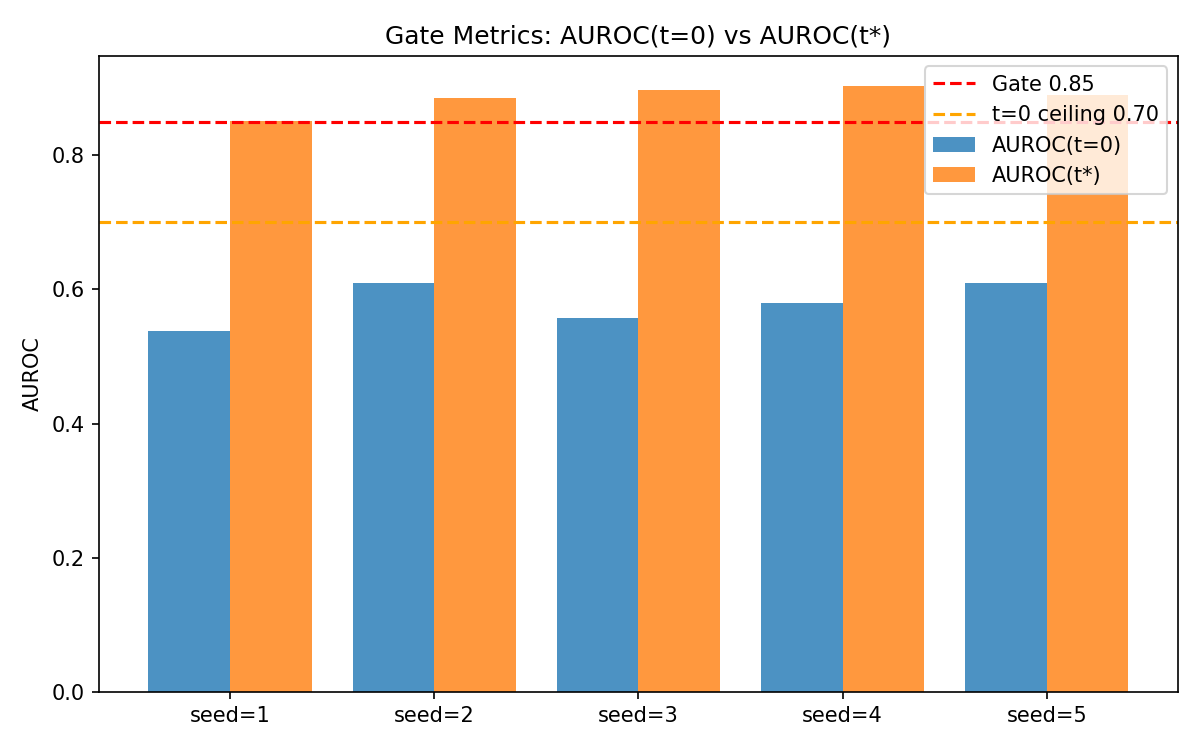
\includegraphics[width=0.8\columnwidth]{figures/fig1_gate_metrics.png}
\caption{AUROC at epoch 0 and at $t^*$ per seed, with gate thresholds (dashed lines). 4/5 seeds pass the H-E3 gate (AUROC$(t^*)\geq$0.85 and AUROC$(t{=}0)<$0.70).}
\label{fig:gate_metrics}
\end{figure}

\begin{figure}[h]
\centering
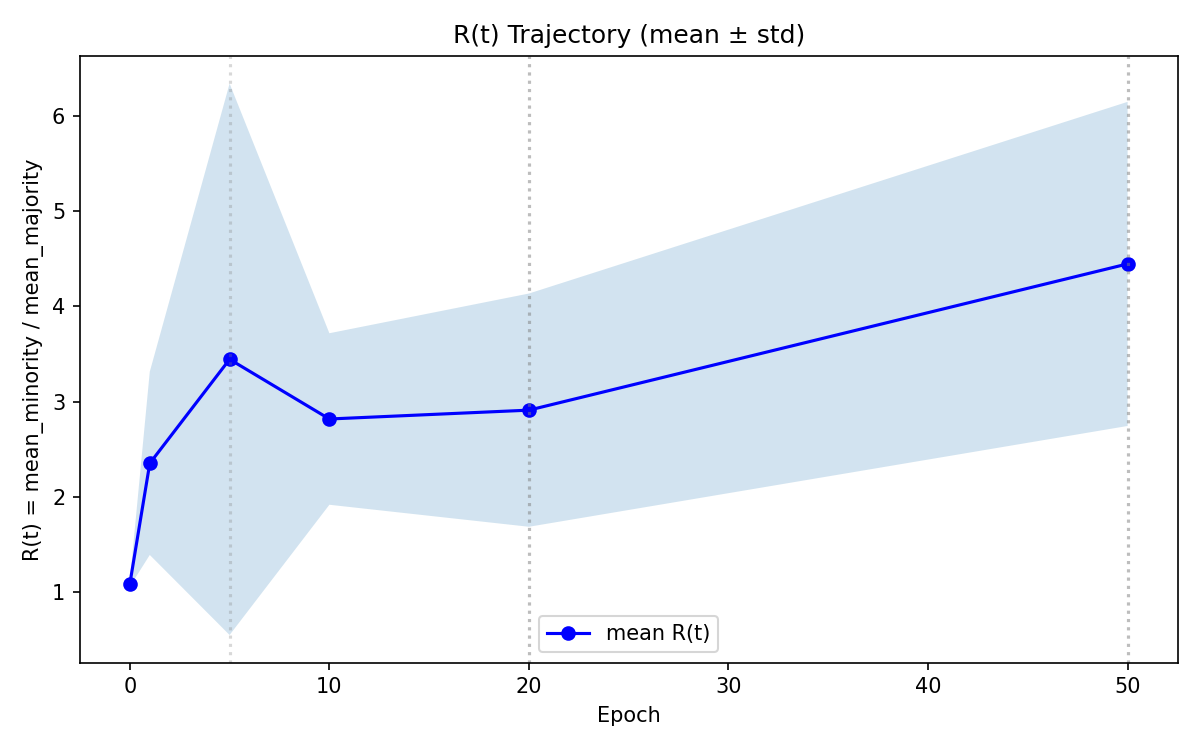
\includegraphics[width=0.8\columnwidth]{figures/fig2_R_trajectory.png}
\caption{Trace ratio $R(t)$ across training epochs for all 5 seeds. All seeds show $R(t^*)\gg 1$ indicating systematic minority trace elevation.}
\label{fig:R_trajectory}
\end{figure}

\begin{figure}[h]
\centering
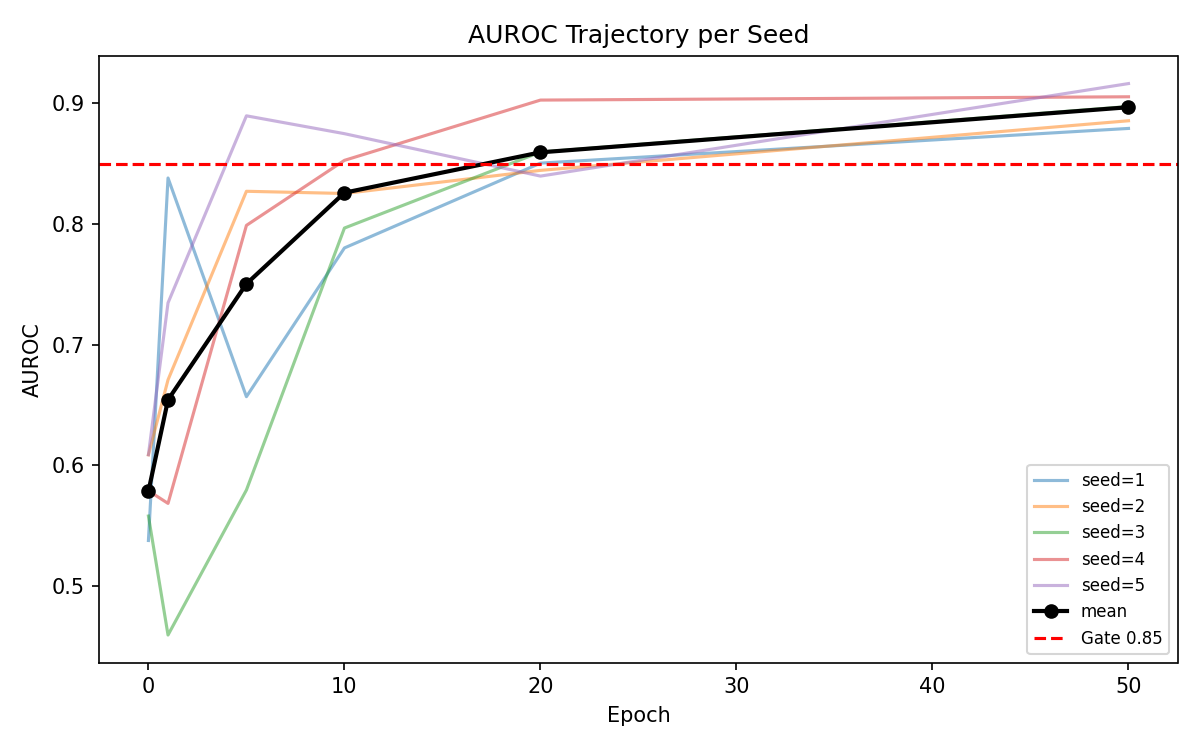
\includegraphics[width=0.8\columnwidth]{figures/fig3_auroc_trajectory.png}
\caption{Full AUROC trajectory across checkpoints $t\in\{0,1,5,10,20,50\}$ for all 5 seeds.}
\label{fig:auroc_trajectory}
\end{figure}

\begin{figure}[h]
\centering
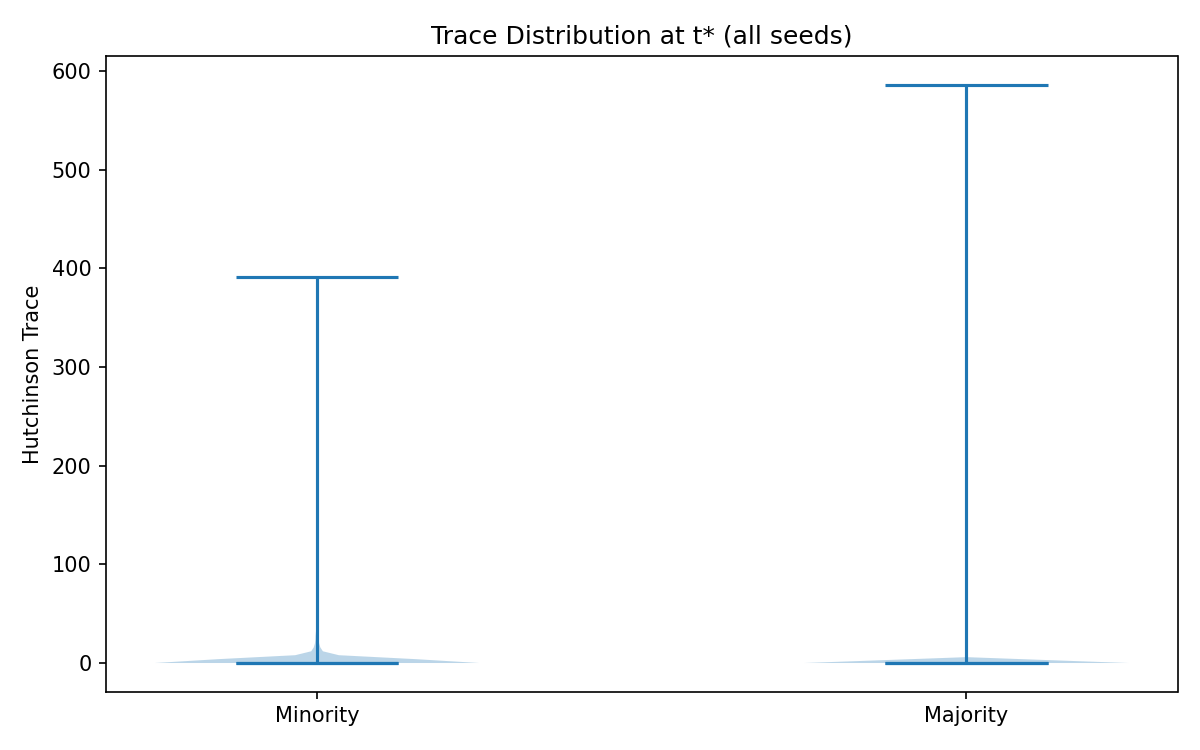
\includegraphics[width=0.8\columnwidth]{figures/fig4_trace_distribution.png}
\caption{Per-sample trace distributions at $t^*$ for minority and majority groups. Minority traces are systematically elevated.}
\label{fig:trace_dist}
\end{figure}

\begin{figure}[h]
\centering
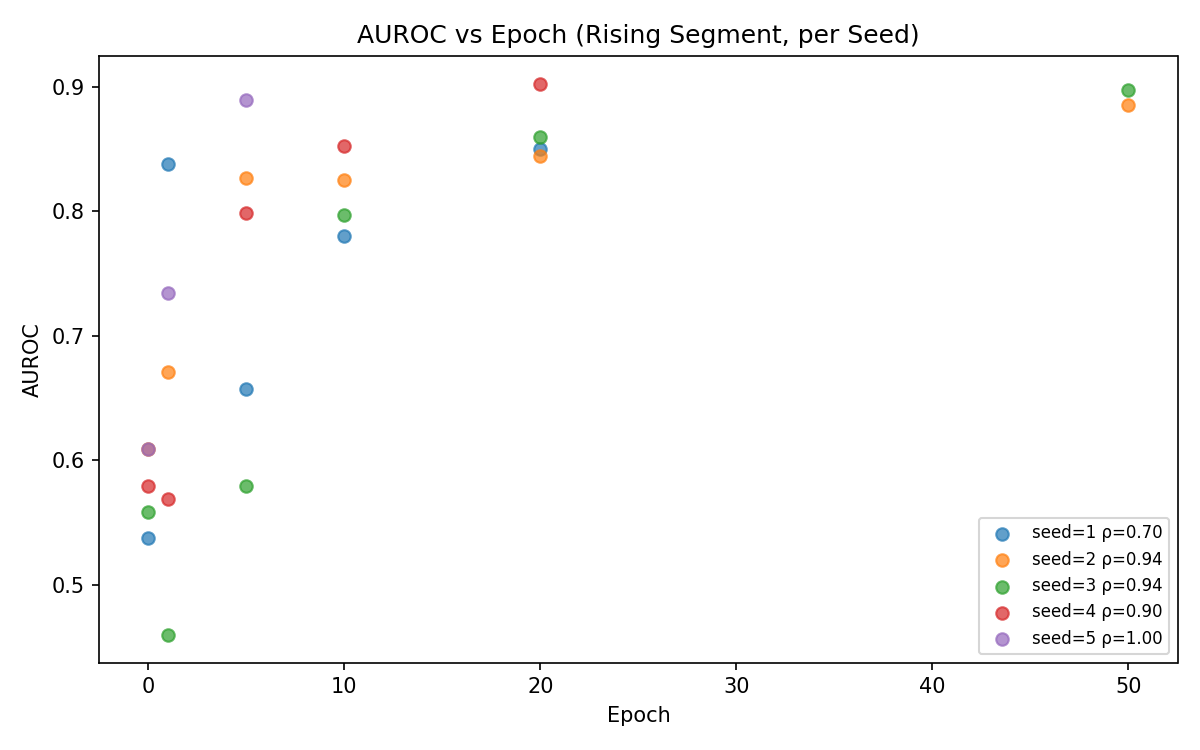
\includegraphics[width=0.8\columnwidth]{figures/fig5_spearman_rising.png}
\caption{Spearman $\rho$ values on the rising AUROC segment per seed.}
\label{fig:spearman}
\end{figure}

\section{Discussion}
\label{sec:discussion}

\subsection{The Dual Finding: Existence Without Expected Mechanism}

The core finding of this work is a dual result. The trace signal is real: per-sample last-fc Hessian trace achieves AUROC$\geq$0.85 for minority membership detection in 4/5 seeds, with the signal being ERM-induced (epoch-0 control). The expected mechanism is absent: at the checkpoint of peak discriminability, minority training confidence is 0.97--1.0 --- indistinguishable from majority in terms of the confidence channel.

This combination --- robust existence result + principled mechanism falsification --- is more informative than either result alone. If only H-E3 had been tested, we would incorrectly attribute the signal to the confidence-differential mechanism by default. If only H-M1 had been tested, we would have no evidence that the trace signal is discriminative at all.

\subsection{What Drives the Trace Signal? The Feature-Norm Channel}

For a linear cross-entropy head with weight $W \in \mathbb{R}^{C\times d}$ and penultimate feature $x_i \in \mathbb{R}^d$:
\begin{equation}
\text{Tr}(H_i^{fc}) \propto \|x_i\|^2 \cdot p_i(1 - p_i)
\end{equation}

At $t^*$, $p_i(1-p_i)\to 0$ for all training samples (both minority and majority). The confidence term is inactive. The only surviving candidate driver of the trace asymmetry is $\|x_i\|^2$ --- systematic differences in the $\ell_2$ norm of the penultimate-layer feature representation between minority and majority samples.

\cite{labonte2024spectral} provide a group-level prediction consistent with this interpretation: minority group covariance matrices have larger spectral norm than majority groups within the same class --- a prediction of systematic feature-norm elevation for minority samples. Our finding extends this from the group-level covariance setting to the per-sample trace trajectory, and identifies $\|x_i\|^2$ as the specific channel that would need to show differential behavior.

\textbf{This interpretation is a candidate, not a verified claim.} We have not directly measured penultimate-layer norms $\|x_i\|^2$ per sample or confirmed that minority norms exceed majority norms. Verifying this --- by measuring feature norms at $t^*$ and correlating them with trace ranks --- is the primary direction for future mechanistic investigation (see Section~\ref{sec:limitations}).

\subsection{Relation to LaBonte \& Muthukumar 2026 Phase I/II Theory}

\cite{labonte2026phase} prove for an XOR spurious feature model that SGD learns the spurious feature first (Phase I), then the core feature (Phase II). This predicts that during Phase I, minority samples (which lack the spurious feature) remain near the decision boundary, keeping $p_{\text{minority}}(t)\approx 0.5$ while $p_{\text{majority}}(t^*)>0.9$.

Our results show that on ResNet-50 on Waterbirds, a transient version of this is real at epoch 1 but does not persist to $t^*$. ERM memorizes minority training samples --- driving their training confidence to $\geq 0.97$ --- before the trace ratio $R(t)$ reaches its maximum. The mechanism operates on a different timescale than $t^*$.

Two non-exclusive interpretations: (1) the Phase I window for ResNet-50 on Waterbirds closes very quickly (by epoch 5 at the latest), so the confidence differential is genuinely transient; (2) ResNet-50 with ImageNet pretraining can memorize minority samples via the pretrained feature representation even without the spurious correlation, and this memorization outpaces the Phase I dynamics. Distinguishing these requires holding constant the spuriosity level and model capacity, which we leave for future work.

\subsection{Limitations}
\label{sec:limitations}

\textbf{Scope:} All experiments use ResNet-50 on Waterbirds v1.0 with 95\% spuriosity. Generalization to other architectures (ViT, ResNet-18), datasets (CelebA, MultiNLI), or spuriosity levels is unknown.

\textbf{Mechanism unverified:} The feature-norm channel ($\|x_i\|^2$) is a candidate explanation, not a verified claim. The next step is to directly measure per-sample penultimate-layer norms at $t^*$ and test whether minority norms exceed majority norms at the same rank order as Hessian traces.

\textbf{No DFR application:} We have not tested whether the trace signal, used as a sample-weight or resampling guide for last-layer retraining (analogous to JTT upweighting), improves worst-group accuracy. The existence result (AUROC$>$0.85) is necessary but not sufficient for practical WGA improvement.

\textbf{Training-set confidence only:} The H-M1 mechanism test uses training-set confidence. A different test --- measuring confidence on held-out samples --- might show a different boundary-condition pattern.

\textbf{Seed 1 failure:} One seed (seed 1) fails the H-E3 gate due to a non-monotone AUROC trajectory (Spearman $\rho{=}0.70$). This may reflect stochastic optimization dynamics at a specific random initialization rather than a systematic failure mode.

\subsection{Implications for Annotation-Free Minority Detection}

Our work identifies per-sample last-fc Hessian trace as a candidate second-order annotation-free proxy for minority group membership --- the first such signal to achieve AUROC$>$0.85 on Waterbirds without group labels, with a verified epoch-0 control ruling out pretrained-artifact confounds.

The key practical questions remaining are: (1) does the trace proxy translate to WGA improvement via DFR-style last-layer retraining; (2) does the signal generalize beyond Waterbirds; (3) what is the minimal computation needed. If the feature-norm mechanism is confirmed, it would also suggest that directly measuring $\|x_i\|^2$ as an annotation-free proxy might be cheaper than the full Hutchinson computation --- a simplification worth testing.

\section{Conclusion}
\label{sec:conclusion}

We set out to test whether the curvature of the ERM loss surface --- measured as per-sample Hessian trace of the last fully-connected layer --- reveals minority group membership without group annotations. It does: 4/5 random seeds achieve AUROC$\geq$0.85 at the epoch of maximum trace ratio, with the epoch-0 control confirming that the signal is created by ERM training on Waterbirds, not inherited from ImageNet pretraining.

We then set out to understand why. We expected that ERM's spurious feature exploitation would keep minority training samples near the decision boundary (Phase I confidence-differential mechanism), with the $p_i(1-p_i)$ confidence channel elevating their Hessian traces. This expected mechanism is absent: minority training confidence saturates to $\geq$0.97 at $t^*$, identical to majority. The signal is robust; its original mechanistic explanation is not.

This is not a failure. It is a precise scientific finding that eliminates one mechanism and identifies the right one to test next: the feature-norm channel ($\|x_i\|^2$). \cite{labonte2024spectral}'s spectral imbalance result --- that minority group covariance matrices have larger spectral norm than majority groups --- predicts that minority per-sample feature norms are systematically elevated, and with the confidence channel inactive, this is the remaining candidate. Testing it directly (measuring penultimate-layer norms at $t^*$ and correlating with trace ranks) is the primary next step.

The practical path forward is equally clear: test whether the trace proxy, used to guide annotation-free last-layer retraining (DFR-style), improves worst-group accuracy on Waterbirds. The existence result (AUROC$>$0.85) establishes the signal quality that makes this worth testing; the mechanism result identifies what signal the proxy is actually capturing.

A second-order perspective on spurious feature reliance --- one that asks how ERM differentially shapes the loss landscape curvature around training samples, not just how it classifies them --- opens a class of annotation-free minority detectors that first-order signals cannot replicate. This paper establishes the empirical foundation and the mechanistic question for that class.

\subsection*{Broader Impact}

This work advances annotation-free methods for identifying minority groups in machine learning training data. The ability to detect spuriously correlated minority samples without group labels could reduce the annotation burden for fairness-motivated model corrections. However, the same signal could in principle be used to identify and selectively filter minority samples in adversarial settings. We encourage future users of this method to apply it in contexts where minority detection supports, rather than undermines, equitable model performance.


\bibliographystyle{plainnat}
\bibliography{references}

\end{document}
